\textbf{CFL-condition}:
For an explicit scheme for the differential equation $\partial h/\partial t + \lambda \partial h/ \partial x = 0$ the CFL-condition is $C = \left | \lambda \frac{\Delta t}{\Delta x}\right| < 1$.
%
However, we want to simulate the behaviour of \eqref{eq:rescaled_conservation_of_matter}, which can be written as
%
\begin{equation}
    \partial_th+\lambda (m+2)h^{m+1} \frac{\dif}{\dif{x}}h = q.
\end{equation}
%
If we assume that $q$ is sufficiently small, thus locally constant, this term can be neglected. Since this equation is scaled, a likely bound for the maximum value of the height $h_{\text{max}} < 2$, so the CFL-condition becomes:
\begin{equation*}
    C = \left | \lambda (m+2) h_\text{max}^{m+1} \frac{\Delta t}{\Delta x}\right| =\left | \kappa h_{\text{max}}^{m+1} \frac{\Delta t}{\Delta x}\right| < \left | \kappa 2^{m+1} \frac{\Delta t}{\Delta x}\right| < 1
\end{equation*}
%
\textbf{Numerical Schemes:}\\
The following schemes were applied for the numerical implementation.
%
Finite volume:
%
\begin{align} \label{eq:finite_volume_scheme}
    \begin{split}
        & h_i^{j+1} \approx h_i^{j} + \frac{\Delta t}{2} \left (q_i^j + q_{i+1}^j \right) + \frac{\lambda \Delta t}{\Delta x} \left( \left [h_i^j\right]^{m+2} - \left[h_{i+1}^j\right]^{m+2}\right) \\
    \end{split}
\end{align}
%
Upwind scheme:
%
\begin{align} \label{eq:upwind_scheme}
\begin{split}
    & h_i^{j+1} \approx h_i^j + \frac{\Delta x}{\Delta t} \left( \Delta x q_i - \kappa \left( h_i^j \right)^{m+1} \left (h_{i}^j - h_{i-1}^j \right) \right)
    \end{split}
\end{align}
%
%%%%%%%%%%%%%%%% BEGIN COMMENT %%%%%%%%%%%%%%%%%%%%
\begin{comment}
A simplified model for q will be used

\begin{verbatim}
    q|
     |
     |
q_0  |___________________________
     |                          | \
     |                             \
     |                          |   \
     |_______________________________\    |______|__________
     |                          x_s   \   x_f
     |                                 \
     |                                  \
\end{verbatim}



The toe of the glacier remains t be solved for.
%
Now apply the finite volume method for this problem. Sub-divide the x-domain of interest $[0,L]$
%

\begin{align*}
 \begin{split}
     0 &= x_1 < x_2 < \dots < x_n = L\\
     \Delta x :&= x_{i+1} -x_i \Rightarrow \quad \text{constant step length}
 \end{split}   
\end{align*}

Now solve for numerically:
\begin{equation*}
    \begin{cases}
    & \frac{\dif}{\dif{t}}\int_{x_{i}}^{x_{i+1}} h(x,t) \dif{x} + j(x_i, t) - j(x_{i+1},t) = \int_{x_{i}}^{x_{i+1}} q(x,t) \dif{x} \\
    & j(x,t) := \lambda h^{m+2}
    \end{cases}
\end{equation*}

Now numerical approximations:
\begin{align*}
    \begin{split}
        & \frac{\dif}{\dif{t}} \left [h_i^j \Delta x \right] + \lambda \left[\left(h_i^j\right)^{m+2} - \left(h_{i+1}^j\right)^{m+2} \right] \approx \Delta x \cdot q_i^j \\
        & \frac{\Delta x}{\Delta t} \left (h_i^{j+1} - h_i^j\right) + \lambda \left[\left(h_i^j\right)^{m+2} - \left(h_{i+1}^j\right)^{m+2} \right] \approx \Delta x \cdot q_i^j \\
        & h_i^{i+1} \approx h_i^{i} + \frac{\Delta x}{\Delta t} \left (\Delta x\cdot q_i^j - \lambda \left[\left(h_i^j\right)^{m+2} - \left(h_{i+1}^j\right)^{m+2} \right]  \right), \\
    \end{split}
\end{align*}

where we can choose $q_0$ and $\left(h_0^{j}\right) = $ const.
%
Given $q(x)$, find $h(x)$ steady state:
\begin{align*}
    \begin{split}
        h(x) &= \frac{1}{\lambda^{1/m+2}}\left(\int_0^xq(y)\dif{y} +C\right)^{1/m+2} \\
        h(0) &= \left(\frac{c}{\lambda}\right)^\frac{1}{m+2} \Rightarrow C = \lambda h(O)^{m+2} \\
        h(x) &= \left[\frac{1}{\lambda}\left( \int_0^xq(y)\dif{y} +\lambda h(O)^{m+2}\right)\right]^{1/m+2} \\
        h(x) &= \left(\frac{1}{\lambda} \int_0^xq(y)\dif{y} \right)^{1/m+2} + h(0) \\
    \end{split}
\end{align*}
%
\red{Her skjønner jeg ikke helt rekkefølgen på ting... -Johan}
%
\begin{align*}
    \begin{split}
        \int \dif f(x) &= \int g(x) \dif{x} \qquad Q(0) = f(0) \\
        f(x) &= \int^x g(y) \dif{y} + \\
        \int g(x) \dif{x} &= G(x) \\
        \int_a^x g(y) \dif{y} &= G(X) - G(a)
    \end{split}
\end{align*}
%
\red{**FIGUR**}
%
\begin{align*}
    \begin{split}
        q_0 x_0 &= q_0 + \int_0^{x_F-x_S} \\
        \frac{q_0 x_s - q_0}{\frac{1}{2}(x_F - x_S)^2} &= \alpha \\
        \alpha &= \frac{2q_0 (x_s - 1)}{(x_F - x_S)^2}
    \end{split}
\end{align*}
%
\red{**FIGUR**}
%
\begin{align*}
    \begin{split}
        & q_0 x_S + \int_0^{x_F - x_S}(q_0 + \alpha x) \dif{x} = 0\\
        & q_0 x_S + \left[q_0 x + \frac{1}{2}\alpha x^2\right]_0^{x_F - x_S} = 0\\
        & q_0 x_S + q_0 (x_F - x_S) + \frac{1}{2}\alpha (x_F - x_S)^2 = 0\\
    \end{split}
\end{align*}
%
\red{**FIGUR**}
%
\begin{align*}
    \begin{split}
        \alpha &= \frac{-2(q_0 x_F + h_0)}{(x_F - x_0)^2} \\
        \lim_{t\rightarrow \infty} k &= 0 \\
        \frac{\partial u}{\partial t} &= -u
    \end{split}
\end{align*}
%
\begin{align*}
    \begin{split}
        q_0 x_S + \int_0^{x_F - x_S}(\alpha x + q_0) \dif{x} = 0 \\
        \frac{\partial k}{ \partial t} + \kappa \frac{\dif}{\dif{x}} \left( h_0^{m+1}k\right) = 0 \\
        \lambda \frac{\dif}{\dif{x}} \left( h_0^{m+2}k\right) = q \\
        \frac{\partial k}{ \partial t}+ \kappa \frac{\dif}{\dif{x}}\left( h_0^{m+1}\right) + \kappa h_0^{m+1}\frac{\dif}{\dif{x}}k = 0\\
        \frac{\dif}{\dif{x}} \left(h_0^{m+2} h_0^{-1}\right) = \frac{\dif}{\dif{x}} \left( h_0^{m+2}\right) \frac{1}{h_0} + h^{m+2} \frac{\dif}{\dif{x}}\left( \frac{1}{h_0}\right) = \dots \\
    \end{split}
\end{align*}
%
Now use that $ \frac{\dif}{\dif{x}} \left( h_0^{m+2}\right) = \frac{q}{\lambda}$
%
\begin{align*}
    \begin{split}
        \dots = \frac{q}{\lambda h_0} + h^{m+2} \frac{\dif}{\dif{x}} \left( \frac{1}{h_0}\right)\\
    \end{split}
\end{align*}
%
\begin{align*}
    \begin{split}
        \frac{\partial k}{ \partial t}+ \kappa k \left( \frac{q}{\lambda h_0} + h^{m+2} \frac{\dif}{\dif{x}} \left(\frac{1}{h_0}\right)\right) + \kappa h_0^{m+1} \frac{\dif{k}}{\dif{x}} = 0 \\
        \frac{\partial k}{ \partial t}+ \kappa k \left( \frac{q}{\lambda h_0} + \frac{j(x)}{\lambda} \frac{\dif}{\dif{x}} \left(\frac{1}{h_0}\right)\right) + \kappa h_0^{m+1} \frac{\dif{k}}{\dif{x}} = 0
    \end{split}
\end{align*}
%
\begin{align*}
    \begin{split}
        \frac{\partial k}{\partial t} = - \kappa \frac{\dif{}}{\dif{x}} \left(h_0^{m+1} k\right)
    \end{split}
\end{align*}
%
Which gives the scheme
\begin{align*}
    \begin{split}
        k_i^{j+1} - k_i^j &= - \frac{k}{2\Delta x} \left( \left(h_0^{m+1}\right)_{i+1}^j k_{i+1}^j - \left( h_0^{m+1}\right)_{i-1}^j k_{i-1}^j \right) \\
        k_i^{j+1} &= k_i^j - \frac{k}{2\Delta x} \left( \left(h_0^{m+1}\right)_{i+1}^j k_{i+1}^j - \left( h_0^{m+1}\right)_{i-1}^j k_{i-1}^j \right) 
    \end{split}
\end{align*}
%
Given $h_0, k_0$ and $ \red{(0 <?) }k_0 \ll 1$
%
\begin{align*}
    \begin{split}
        h(x) &= \left(\frac{1}{\lambda} \int_N q^{\text{noe??}} q_0 \right)^{\frac{1}{m+2}} \\
        h(0) &= h_0 = \left(\frac{1}{\lambda}q_0\right)^{1/m+2} \Rightarrow q_0 = (\lambda h_0 )^{m+2}
    \end{split}
\end{align*}
%
\red{**FIGUR**}
%
\begin{align*}
    \begin{split}
        h(x) &= \left(\frac{1}{\lambda} \int q \dif{x} \right)^{\frac{1}{m+2}} \\
        h(x) &= \left(\frac{1}{\lambda} \int_T q \dif{x} + (h_0 \lambda)^{m+2} \right)^{\frac{1}{m+2}}
    \end{split}
\end{align*}
%
Tongue:
\begin{align*}
    x_F = \int_0^{x_F} q(y) \dif{y} = 0 \\
\end{align*}
%
$\dots$
%
\begin{align*}
    q_0 x_F + \frac{1}{2} \alpha (x_F - x_S)^2 &= -\frac{1}{\lambda} h_0^{m+2} \\
    \alpha &= \frac{-2 \left(q_0 x_F + \frac{1}{\lambda} h_0^{m+2}\right)}{(x_F - x_S)^2}
\end{align*}
%
$\dots$
%
\begin{align*}
      -\lambda h(0)^{m+2}&= q_0 x_F + \frac{1}{2} \alpha (x_F - x_S)^2  \\
    \alpha &= \frac{-2 \left(q_0 x_F + \lambda h(0)^{m+2}\right)}{(x_F - x_S)^2}
\end{align*}
\end{comment}
%%%%%%%%%%%% END COMMENT %%%%%%%%%%%%%%%%

The explicit expressions for the flow field are shown in \eqref{eq:explicit_u_h} and \eqref{eq:explicit_v_h}. The flow field within the glacier can be computed by evaluating these equations on grid points within the glacier. The derivative in \eqref{eq:explicit_v_h} is approximated using central differences. Forward and backwards differences are used on the boundaries of the grid.

The stationary glacier for a given accumulation rate is found using the method described in \red{reference to relevant section or equation}.

\begin{figure}[h]
    \centering
    \begin{subfigure}[b]{0.4\textwidth}
        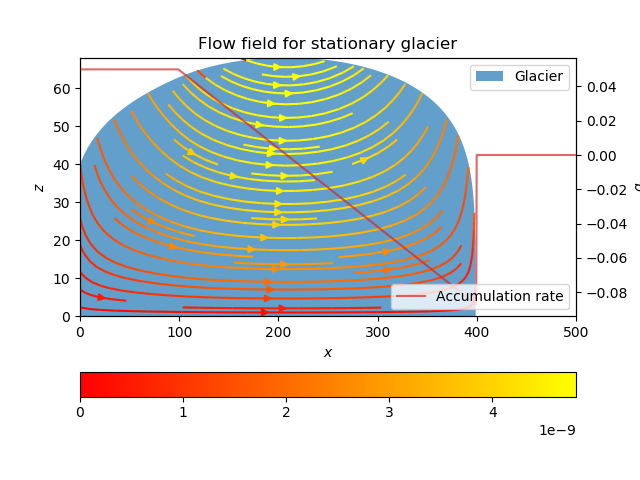
\includegraphics[width=\textwidth]{report/images/flow_field_linear_production.png}
        \caption{Accumulation rate as specified in \red{a}}
        \label{fig:linear}
    \end{subfigure}
    \begin{subfigure}[b]{0.4\textwidth}
        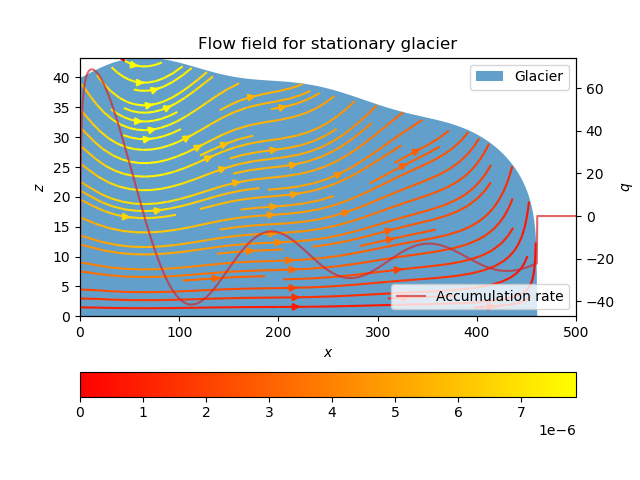
\includegraphics[width=\textwidth]{report/images/flow_field_arbitrary_production.png}
        \caption{Arbitrary accumulation rate}
        \label{fig:arbitrary}
    \end{subfigure}
    \caption{Stationary glaciers with height on left axis, accumulation rate on right axis and stream lines for the internal flow field}\label{fig:animals}
\end{figure}

The flow field for the production rate $q(x) = 5\sin(\frac{x}{25})\frac{1}{2(x + 1)} - 0.01$ is shown in figure \ref{fig:arbitrary}.

The flow field for a production rate as shown in \red{Description of accumulation rate} is shown in figure \ref{fig:linear}.